\documentclass{article}
\usepackage{lmodern}
\usepackage[T1]{fontenc}
\usepackage[english,activeacute]{babel}
\usepackage{mathtools}
\usepackage{biblatex}
\usepackage{csquotes}
\usepackage{graphicx}

\setcounter{tocdepth}{5}
%\setcounter{secnumdepth}{5}

\title{User Behavior Analysis in Campus Area Networks through Kohonen Self Organizing Feature Maps}

\author{Nelson Victor Cruz Hern\'andez }

\date{May 2017}

\begin{document}

\maketitle






\section{Introduction} % level 1
Inbounds

\subsection{Background} % level 2

\subsection{Justification} % level 2

\subsection{Problem} % level 2

\subsection{Hypothesis} % level 2

\subsection{Objectives} % level 2

\subsubsection{General Objectives} % level 3

\subsubsection{Particular Objectives} % level 3







\section{State of the Art} % level 1

\subsection{Machine Learning Algorithms and Computer Security} % level 2

\subsection{Profiling  and User classification} % level 2






\section{Theorical framework} % level 1

\subsection{Proxy} % level 2

\subsection{Machine Learning algorithms}	 % level 2

\subsubsection{Learning methods} % level 3

\paragraph{Supervised Training Methods} % level 4
Obtain the information from "Artificial Neural Networks An introduction Kevin L. Priddy and Paul E. Keller" Chapter 2.1

\paragraph{Unsupervised Training Methods} % level 4
Obtain the information from "Artificial Neural Networks An introduction Kevin L. Priddy and Paul E. Keller" Chapter 2.3
                                                                                                                                                                                                                                                                                                                                                                                                                                                                                                                                                                                                                                                                                                                                                                                                                                                                                                                                                                                                                                                                                                                                                                                                                                                                                                                                                                                                                                                                                                                                                                                                                                                                                                                                                                                                                                                                                                                                                                                                                                                                                                                                                                                                                                                                                                                                                          \subsubsection{Gaussian function} % level 3

\subsection{Self-organizing Maps} % level 2
The concept, design, and implementation techniques of Self-Organizing Maps are described in detail in [25]. The Self-Organizing Map algorithm performs a nonlinear, ordered, smooth mapping of high-dimensional input data manifolds onto the elements of a regular, low-dimensional array [25]. The algorithm converts non-linear statistical relationships between data elements in a high-dimensional space into geometrical relationships between elements in a two-dimensional map (lattice), called the Self-Organizing Map (SOM)[1]. A SOM can then be used to visualize the clusters, of an input space. Each element at SOM is a neuron, and is a representation of a multidimensional vector with a cartographic position denoted with x and y. If elements in the input space are characterized using k parameters and represented by k-dimensional vectors, each neuron in the SOM lattice is also specified as k-dimensional vector.

\subsubsection{Learning} % level 3
In the learning or training phase, the neurons in SOM try to model the input space. 
Self-Organizing Maps differ from from other artificial neuronal networks as they apply competitive learning as opposed to error-correction learning, such as back propagation with gradient descent, also apply a cooperative schema, using a neighborhood function to preserve topological properties of the input surfface.

\paragraph{Competitive} % level 4
Each element of the train data set is shown to every neuron in the SOM lattice. Each neuron has a response, to the shown element, the neuron that gives the best response is called the "winning" neuron, and takes it's k dimensional values adjusted so in the future it responds better to a similar input.

\paragraph{Cooperative} % level 4
Once the winning neuron has adjusted it's k dimensional values, it's neighborhood is calculated, and all neurons that are in the vicinity  of the winning neuron adjust their k dimensional values so in the future they respond better  to a similar input.

\paragraph{Distance Measure} % level 4
Suitable distance measure should be stablished in order to find the winner neuron. Two common used distance measures are dot-product measure and euclidean distance.

In order to use dot-product measure lattice neurons and train element vectors should be normalized. Normalization of a vector $V(v_1, v_2, v_3,...,v_n)$ is a process of transforming it's components into
$(\frac{v_1}{\sqrt{v_1^2+v_2^2+...+v_n^2}},
\frac{v_2}{\sqrt{v_1^2+v_2^2+...+v_n^2}},
...,
\frac{v_n}{\sqrt{v_1^2+v_2^2+...+v_n^2}}
)$
 so that the modules of the normalized vector is unity. The dot-product of the input vector is calculated against all the neurons in the lattice, where dot-product of two vectors $Y(x_1, x_2, x_3,..., x_n)$ and $Z(z_1, z_2, z_3,..., z_n)$ is defined to be $x_1 \cdot z_1 + x_2 \cdot z_2 + x_3 \cdot z_3 + ... + x_n \cdot z_n$. Using this measure means that the winner neuron is the one that gives the maximum dot-product value.

In the other hand euclidean distance measure does not need vector normalization and the winner neuron is defined for the minimum obtained distance. For two vectors $Y(y_1,y_2,...,y_n)$ and $Z(z_1,z_2,...,z_n)$ euclidean distance is given by $\sqrt{(z_1-y_1)^2 + (z_2-y_2)^2 + ... + (z_n-y_n)^2}$.

\paragraph{Neighborhood Function} % level 4

\paragraph{Learning Function} % level 4

\subsection{Redes de Computadoras} % level 2

\subsubsection{Local Area Network (LAN)} % level 3

\subsubsection{Campus Area Network(CAN)} % level 3

\subsubsection{Network topology} % level 3

\subsubsection{OSI Model / TCPIP} % level 3

\subsubsection{Network Security} % level 3

\subsubsection{Intrusion Detection Systems} % level 3






\section{Methodological Development} % level 1






\subsection{Experiment context} % level 2
Experiment was carried out on a Campus Area Network (CAN) that has a 16-bit network and a Windows domain controller, using a HTTP proxy. Among campus applications web and remote apps are included.
Email service is provided by Microsoft Exchange Server which is hosted outside the campus network.
The target users were full-time professors who had a computer with a static IP address and a wireless access with a dynamic IP address.
Five full-time professors (hereafter denoted as users) were selected for the experiment. For each one, real usage traffic was captured (inside and outside campus activities) during a two labor weeks, and then processed.






\subsection{Explanation} % level 2
In this work Self Organizing Maps algorithm is used to create an user pattern inside a Campus Area Network. Experiment is divided in three phases: network data capture, data processing and pattern evaluation.
For network data capture phase a set of raw packages is obtained for each user through tcpdump library, process is explained in [Parres, XX].
For data processing phase each set of raw packages is arbitrary divided in build, train and evaluate sets.
Each set is processed to compress raw packages into chunks of a five minutes window $(t)$ represented by three metrics that involve communication protocol, origin and destination ip and total transmitted bytes.
From obtained build dat set, a fixed number of elements $(n)$ is randomly selected, this number defines the size of the Self Organizing Map lattice $(n x n)$.
For lattice training, a fixed number of elements $(e)$ is randomly selected from train data set. After ten epochs training Self Organizing Map is considered to be fully trained, as a result an user network behavior pattern is obtained.
Evaluation phase is done by joining different user network behavior patterns in one lattice, similar to a blanket filled of patches in which each patch is represented by an user network behavior pattern, creating what we define as the organization pattern. An organization evaluation set is build by all the user evaluation sets that belong to each user that conforms the organizational pattern. Each element of the organization evaluation set is shown to the organization pattern, resulting best matching unit is compared against the original user of the shown element to the lattice. Correct match of the user attribute of the shown element and user attribute of the best matching verifies that the shown element is able to recognize it's original user among others. Fig. 1 shows an schema of the complete process.

	\begin{center}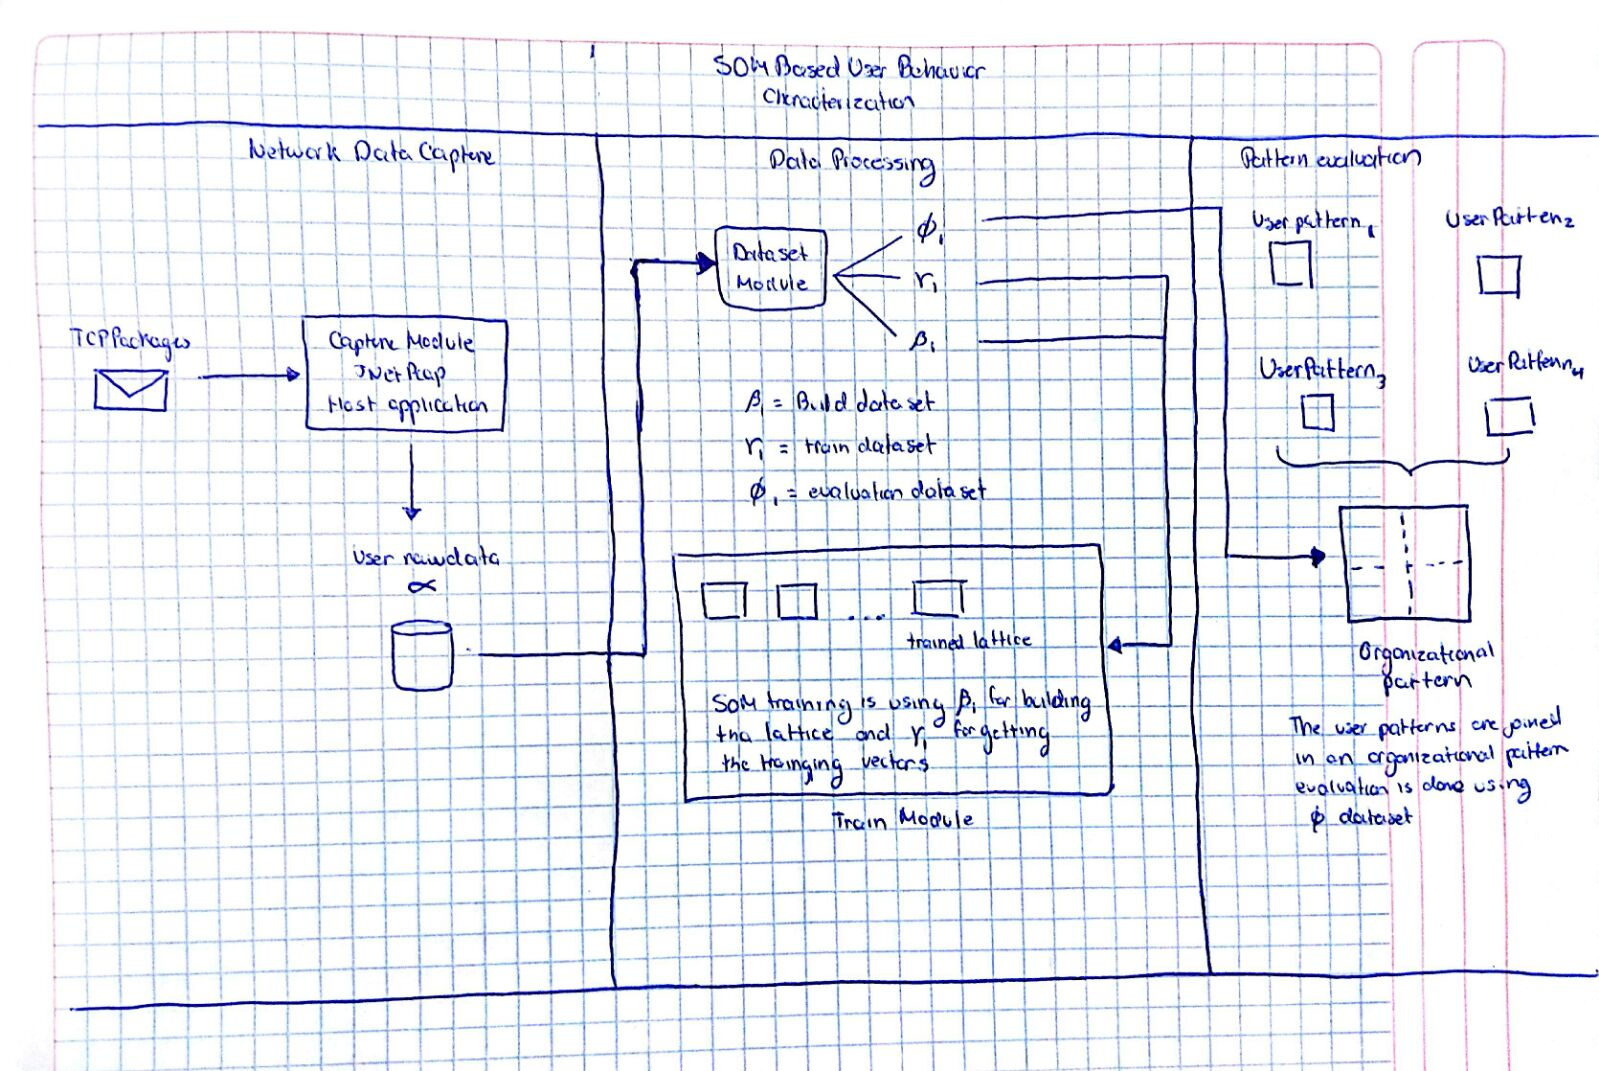
\includegraphics[scale=0.2]{fig-two} \end{center}

For each phase in the process one or more modules were build, each module's output is used as an input for the next the phase corresponding module.






\subsubsection{Network data capture} % level 3
Network data capture phase duration was of two labor weeks,  in which network traffic was captured from each user's computer, it's important to say that only the owner has access to the computer and that before starting to capture, we checked that no computers had any malicious software installed.
Capture module was build using jNetPcap, which works as a client application that once installed enables to capture continuously user network data in an IP packet format and save it in files of twenty megabytes each, naming them with file's creation timestamp. Average size of complete raw captured traffic for each user is three gigabytes, involving more than four million packages. Each register contains the characterization of a network connection by eight parameters organized as follows: way, origin IP, destination IP, used protocol, local used port, remote used port, total transmitted bytes and timestamp.






\subsubsection{Data processing} % level 3
Data processing phase is divided in four stages: a) divide raw data, b) data set creation, c) Self Organizing Map algorithm implementation and d) User network behavior pattern creation. Two modules were build for it, data set and train module. Data set module involves "divide raw data" and "data set creation" stages and Train module involves "Self Organizing Map algorithm implementation" and "User network behavior pattern creation".



\paragraph{Divide raw data} % level 4
As explained in section 3.3 Self Organizing Map algorithm is a not supervised algorithm due this different information is needed en each phase of the algorithm. Complete user raw captured data ($\alpha$) is divided in three subsets: build package set ($\beta$), train package set ($\gamma$), and evaluation package set ($\phi$). As data captured is divided in files containing continuous user network data, dividing the complete raw data set in subsets, enables having en each subset different days of user behavior. Complete raw data set is divided equally between each subset $\beta \cup \gamma \cup \phi = \alpha$.



\paragraph{Data set creation} % level 4
Using TCP package as the working unit is not possible due the great volume of packages, and time consuming for processing [Reference, XX] each one, instead packages are processed and turned into chunks that will conform a data set. Fig 2 shows the process of dataset creation.

	\begin{center}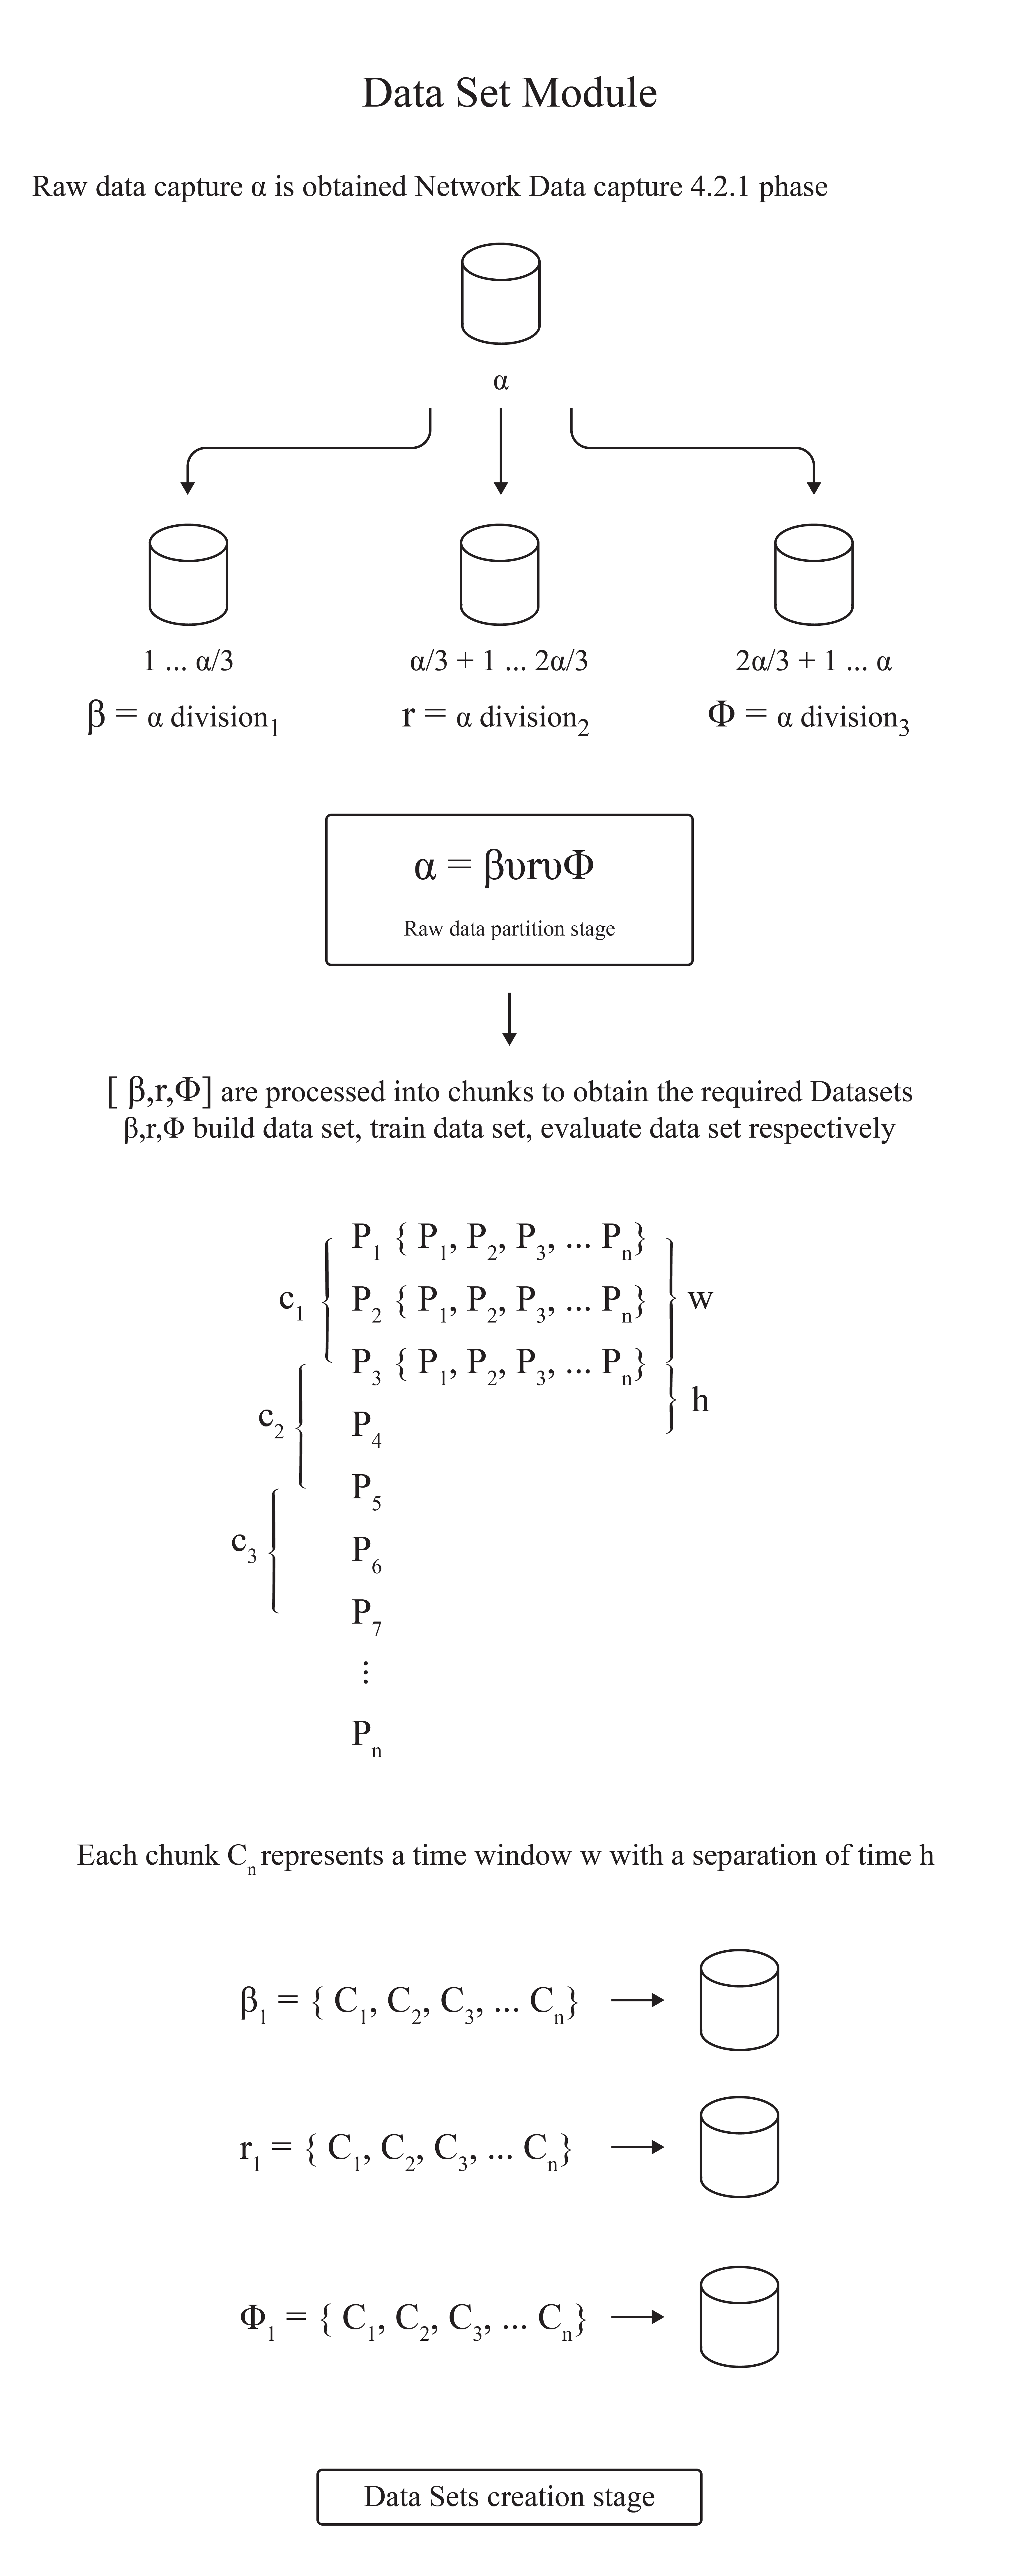
\includegraphics[scale=0.2]{fig-three} \end{center}
	
Each package set ($\beta,\gamma,\phi$) is processed into chunks. A chunk is defined as set of packages with a continuity in their timestamp field $P(p_1,p_2,...,p_n)$ that represent a time window $(t)$ of a fixed time $t_1$. Processing packages as a chunk allows getting a summary of the information sent in a $t_n$ period of time, such as: total bytes sent, total bytes sent through TCP and UDP protocol, total bytes sent for web traffic destination along 80, 443 and 3128 ports and as we are working inside and Campus Area Network total bytes sent to internal destination (same backbone ip, our case 189.230.4.163). This data is condensed into three metrics: a) TCP-UDP metric, represents the ratio between total bytes sent through both protocols and total bytes sent in the chunk , b) Internal IP metric, represents the ratio between total bytes sent to CAN proxy ip and total bytes sent in the chunk and c) Web traffic metric, represents the ratio between data sent through web ports, and and total bytes sent in the chunk.

**** Por trabajar
Para que usamos despues estas metricas
El intervalo entre cada chunk
Data as total bytes sent,  in the $t_1$ time, are obtained,from which collected data is processed and three metrics are obtained and defined as follows: a) TCP-UDP metric
Each data set is created by 1...N data chunks. A data chunk has a set of continuous captured packages P1... P(N) which represents a fixed time window tw of five minutes measured by the packet timestamp, in which three metrics are obtained:
 a) TCP/UDP metric, represents the ratio between total bytes sent through both protocols and total bytes sent in the chunk
 b) bytes to Internal IP metric, represents the ratio between total bytes sent to CAN proxy ip and total bytes sent in the chunk and 
 c) web traffic metric, represents the ratio between data sent through web ports, and and total bytes sent in the chunk. This metrics will be the features which SOM algorithm will arrange the clusters. After tw is processed, a time interval ti of 10 seconds is given to start the data chunk process creation until no more packages are available. Each dataset is conformed by XXX data chunks.
Due the big amount of captured packages and the complexity of processing each packaged as unit in the Self Organizing Map processing packages was needed
**** Por trabajar



\paragraph{Self Organizing Map algorithm implementation} % level 4
For SOM implementation one layer square matrix of 100 x 100 neurons is used. As explained on section 4.0.1 each neuron has an individual feature vector, with specific weights. Our selected vector is conformed by three features, which summarize the total information sent in a range of time $\Delta$t over the network. For winner neuron evaluation euclidean distance is used. Winner and neighbor neurons weights are updated by a gaussian function.
using random initialization


1) Initialize the map using random input vectors of fixed dimension .

2) Searching for the winner neuron.

Select an input vector x randomly from the the training data set.
Search for the neuron ???? which is associated to the closest vector ???? to x which minimize the quantization error |x ? m|.

3) Updating the winner neuron and its neighboring units.
For the winner neuron ???? and its neighbor U ? w, update the features vector using the following equation:
????=????+?????? �?� ???????
where ???? ?? is neighborhood function which is the decreasing function of distance d between ???? and ?????
and ? is the learning rate.

4) Repeat Step 2, Step 3 with decreasing neighborhood function ???? ?? and learning rate ? until the quantization error converges enough or during the pre-defined iterations




\paragraph{User network behavior pattern creation} % level 4
This phase creates a user network pattern that represents its behavior in the network. Many pattern instances could be created from the user build dataset, as elements for creating it are randomly selected. Each neuron of the lattice is represented by an element of the Build Data Set, in which features are the three mentioned metrics in section 5.3.2. The lattice is has an arrange of 100 x 100 neurons, and a stop condition if 10 epochs.

---{Paper [1] ANDSOM Module - Training}






\subsubsection{Pattern evaluation} % level 3
Comparison between two different lattices of the same user

Comparison between different lattices of multiple users

	\begin{center}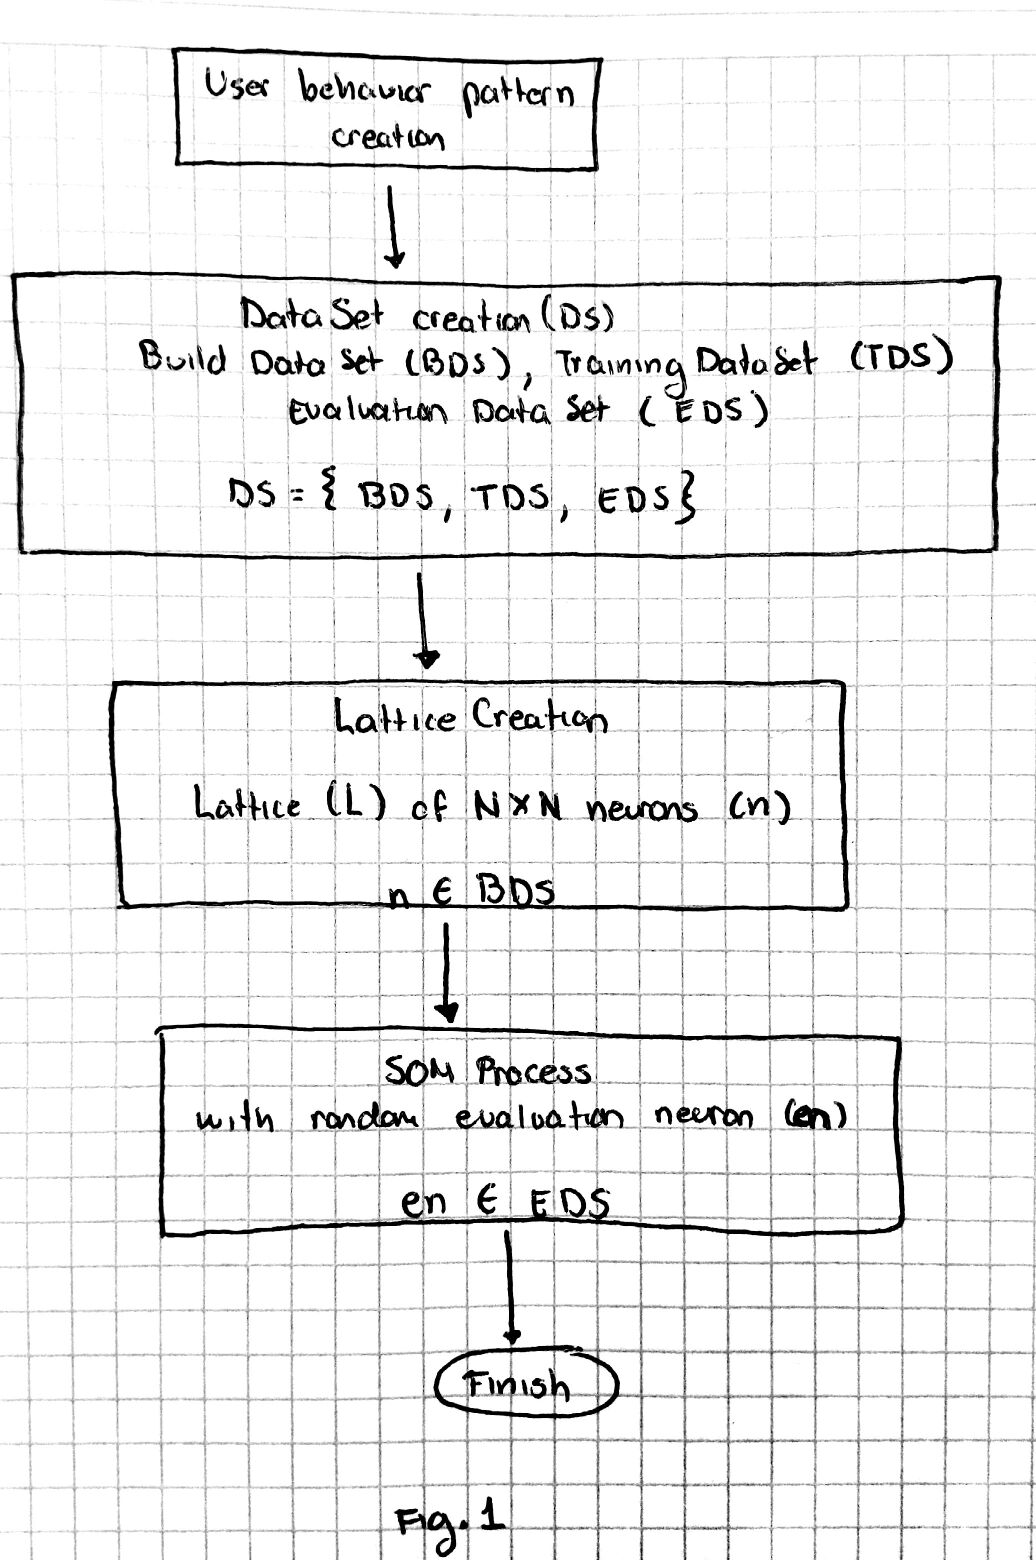
\includegraphics[scale=0.5]{fig-one} \end{center}






\section{Results and Discussion} % level 1
Results presentation, how the results are interpreted, and what we can do with data.
The results will explain, how the user is able to recognize itself in the organization map.






\section{Conclusions} % level 1

\subsection{Future work} % level 2
Due hardware limitation, SOM training is done with ten epochs. A much longer training of about one thousand epochs would give a more precise user pattern, helping in a better user detection in the organization map.
Also formulas are not completely following the standard of a gaussian function so a new implementation would be great.






\section{Bibliography} % level 1
[1] Ramadas, M., Ostermann, S.,  Tjaden, B. Detecting Anomalous Network Traffic with Self-organizing Maps.
[8] Dozono, H., Itou, S., and Nakakuni, M. (2007). Comparison of the adaptive authentication systems for behavior biometrics using the variations of self organizing maps. International Journal of Computers and Communications, 1(4), 108-116.
[25] T.Kohonen. Self Organizing Maps. Springer, third edition, 2001.



\end{document}